\documentclass[12pt]{article}
 
\usepackage[margin=1in]{geometry}
\usepackage{amsmath,amsthm,amssymb}
\usepackage{mathtools}
\DeclarePairedDelimiter{\ceil}{\lceil}{\rceil}
%\usepackage{mathptmx}
\usepackage{accents}
\usepackage{comment}
\usepackage{graphicx}
\usepackage{IEEEtrantools}
 \usepackage{float}
 
\newcommand{\N}{\mathbb{N}}
\newcommand{\Z}{\mathbb{Z}}
\newcommand{\R}{\mathbb{R}}
\newcommand{\Q}{\mathbb{Q}}
\newcommand*\conj[1]{\bar{#1}}
\newcommand*\mean[1]{\bar{#1}}
\newcommand\widebar[1]{\mathop{\overline{#1}}}


\newcommand{\cc}{{\mathbb C}}
\newcommand{\rr}{{\mathbb R}}
\newcommand{\qq}{{\mathbb Q}}
\newcommand{\nn}{\mathbb N}
\newcommand{\zz}{\mathbb Z}
\newcommand{\aaa}{{\mathcal A}}
\newcommand{\bbb}{{\mathcal B}}
\newcommand{\rrr}{{\mathcal R}}
\newcommand{\fff}{{\mathcal F}}
\newcommand{\ppp}{{\mathcal P}}
\newcommand{\eps}{\varepsilon}
\newcommand{\vv}{{\mathbf v}}
\newcommand{\ww}{{\mathbf w}}
\newcommand{\xx}{{\mathbf x}}
\newcommand{\ds}{\displaystyle}
\newcommand{\Om}{\Omega}
\newcommand{\dd}{\mathop{}\,\mathrm{d}}
\newcommand{\ud}{\, \mathrm{d}}
\newcommand{\seq}[1]{\left\{#1\right\}_{n=1}^\infty}
\newcommand{\isp}[1]{\quad\text{#1}\quad}

\DeclareMathOperator{\imag}{Im}
\DeclareMathOperator{\re}{Re}
\DeclareMathOperator{\diam}{diam}
\DeclareMathOperator{\Tr}{Tr}
\DeclareMathOperator{\cis}{cis}

\def\upint{\mathchoice%
    {\mkern13mu\overline{\vphantom{\intop}\mkern7mu}\mkern-20mu}%
    {\mkern7mu\overline{\vphantom{\intop}\mkern7mu}\mkern-14mu}%
    {\mkern7mu\overline{\vphantom{\intop}\mkern7mu}\mkern-14mu}%
    {\mkern7mu\overline{\vphantom{\intop}\mkern7mu}\mkern-14mu}%
  \int}
\def\lowint{\mkern3mu\underline{\vphantom{\intop}\mkern7mu}\mkern-10mu\int}




\newenvironment{theorem}[2][Theorem]{\begin{trivlist}
\item[\hskip \labelsep {\bfseries #1}\hskip \labelsep {\bfseries #2.}]}{\end{trivlist}}
\newenvironment{lemma}[2][Lemma]{\begin{trivlist}
\item[\hskip \labelsep {\bfseries #1}\hskip \labelsep {\bfseries #2.}]}{\end{trivlist}}
\newenvironment{exercise}[2][Exercise]{\begin{trivlist}
\item[\hskip \labelsep {\bfseries #1}\hskip \labelsep {\bfseries #2.}]}{\end{trivlist}}
\newenvironment{problem}[2][Problem]{\begin{trivlist}
\item[\hskip \labelsep {\bfseries #1}\hskip \labelsep {\bfseries #2.}]}{\end{trivlist}}
\newenvironment{question}[2][Question]{\begin{trivlist}
\item[\hskip \labelsep {\bfseries #1}\hskip \labelsep {\bfseries #2.}]}{\end{trivlist}}
\newenvironment{corollary}[2][Corollary]{\begin{trivlist}
\item[\hskip \labelsep {\bfseries #1}\hskip \labelsep {\bfseries #2.}]}{\end{trivlist}}

\newenvironment{solution}{\begin{proof}[Solution]}{\end{proof}}
 
\begin{document}
 
% --------------------------------------------------------------
%                         Start here
% --------------------------------------------------------------
\title{Math 122A Homework 1}
\author{Ethan Martirosyan}
\date{\today}
\maketitle
\hbadness=99999
\hfuzz=50pt
\section*{Introduction}
My name is Ethan Martirosyan, and I am a third-year CCS mathematics student. I have taken 18 mathematics classes at UCSB, all of which were upper division. I have taken the CCS equivalent of 108A and 108B at UCSB, so I have some knowledge of linear algebra. I have not taken any multivariable calculus classes. However, I have taken 118A, 118B, and 118C at UCSB, so I have some experience with undergraduate real analysis. Last quarter, I took 113 (Non-Euclidean Geometry), so I know the basics of hyperbolic geometry.
\newpage
\section*{Problem 1}
\begin{figure}[H]
\centering
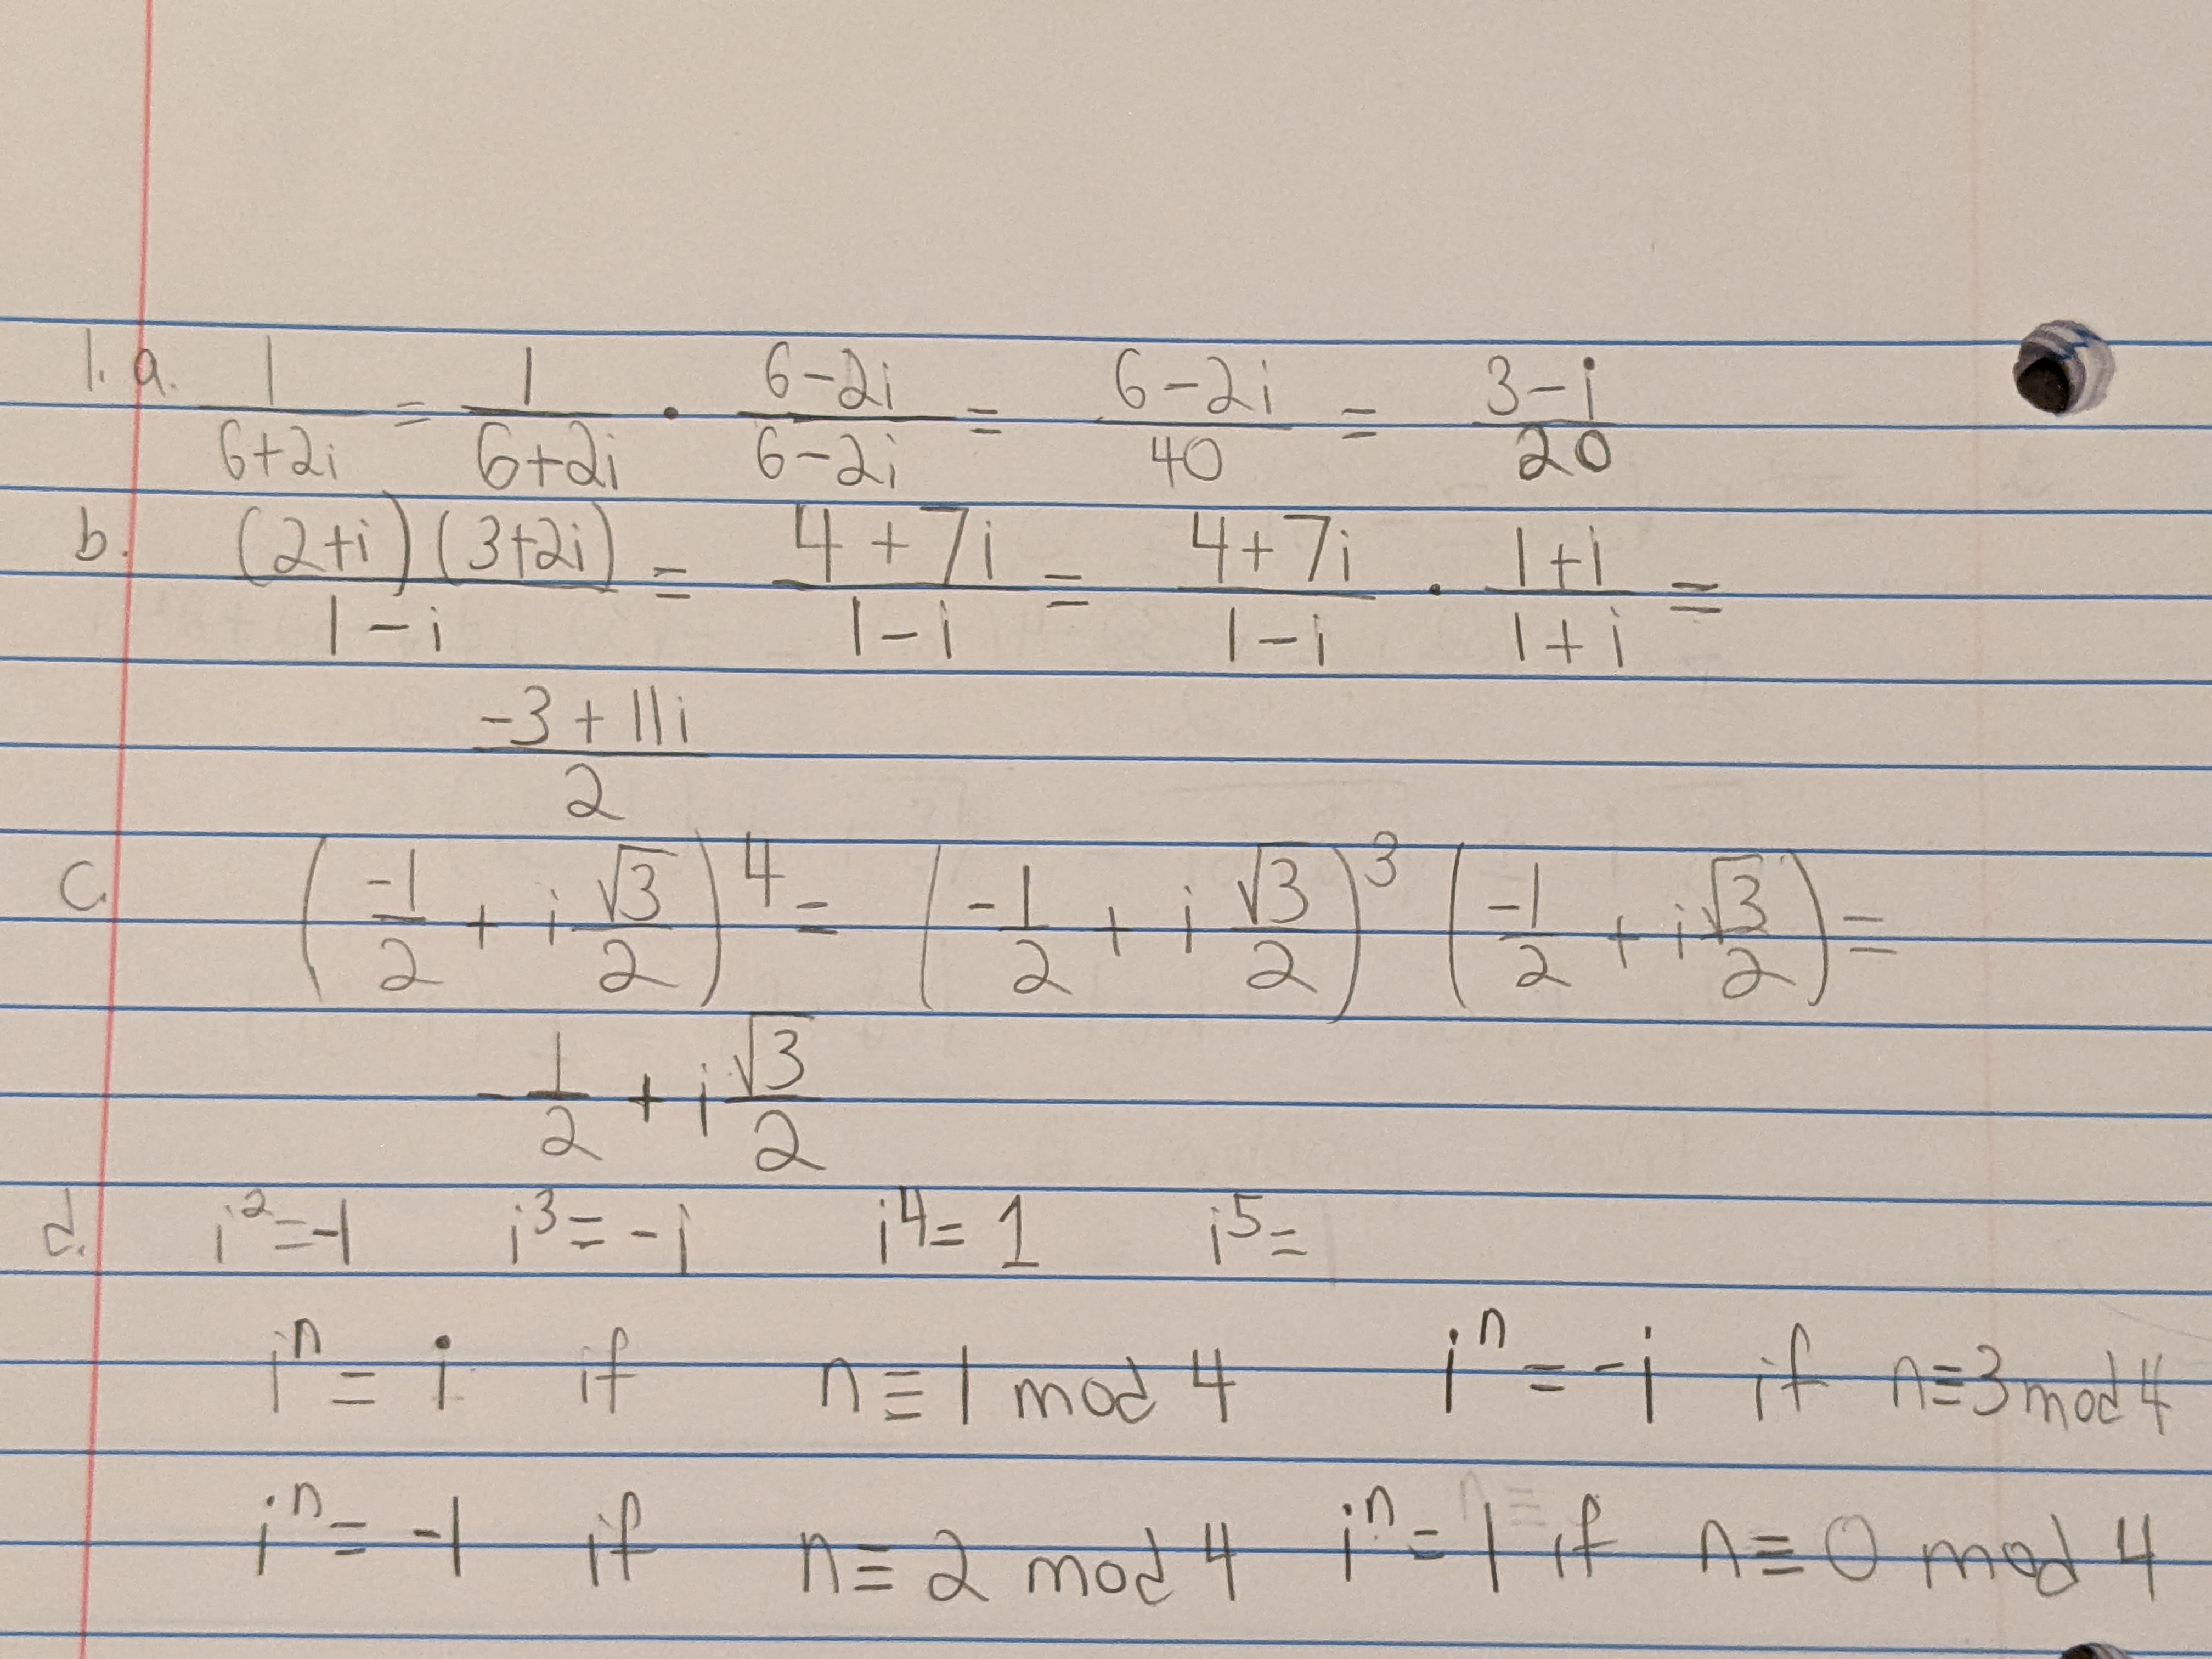
\includegraphics[width=\textwidth]{1}
\end{figure}
\newpage
\section*{Problem 2}
\begin{figure}[H]
\centering
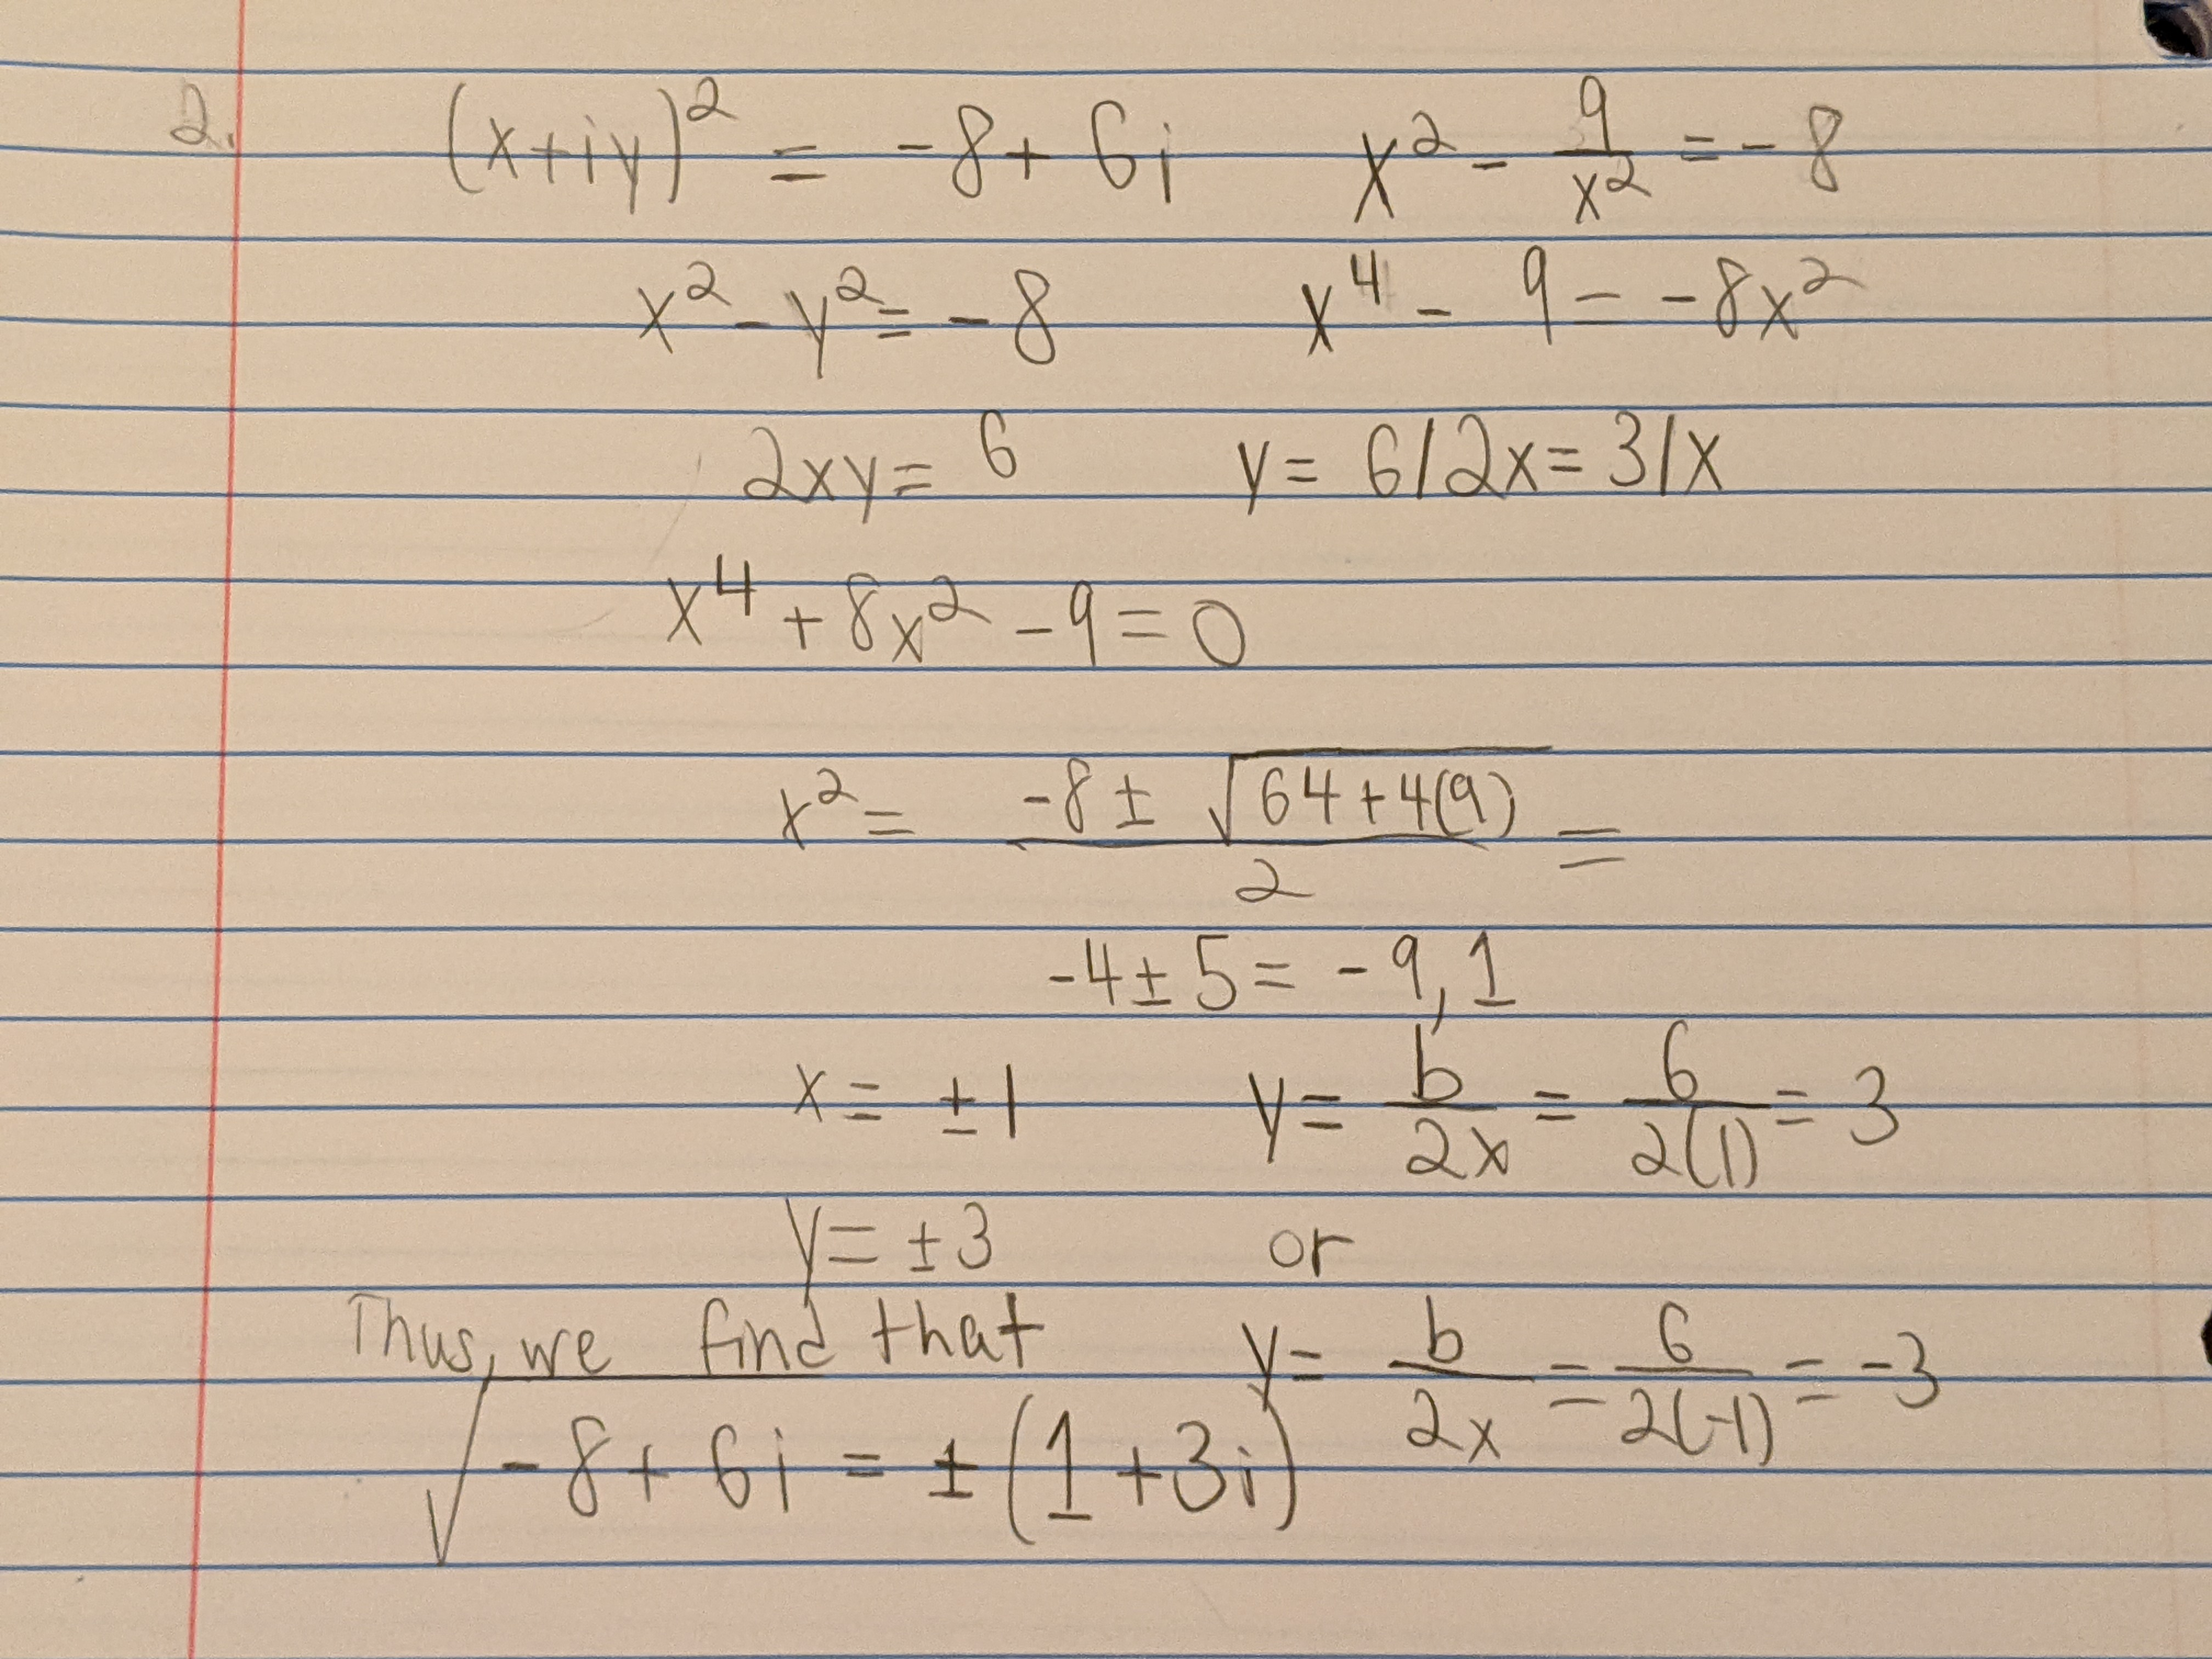
\includegraphics[width=\textwidth]{2}
\end{figure}
\newpage
\section*{Problem 3}
\begin{figure}[H]
\centering
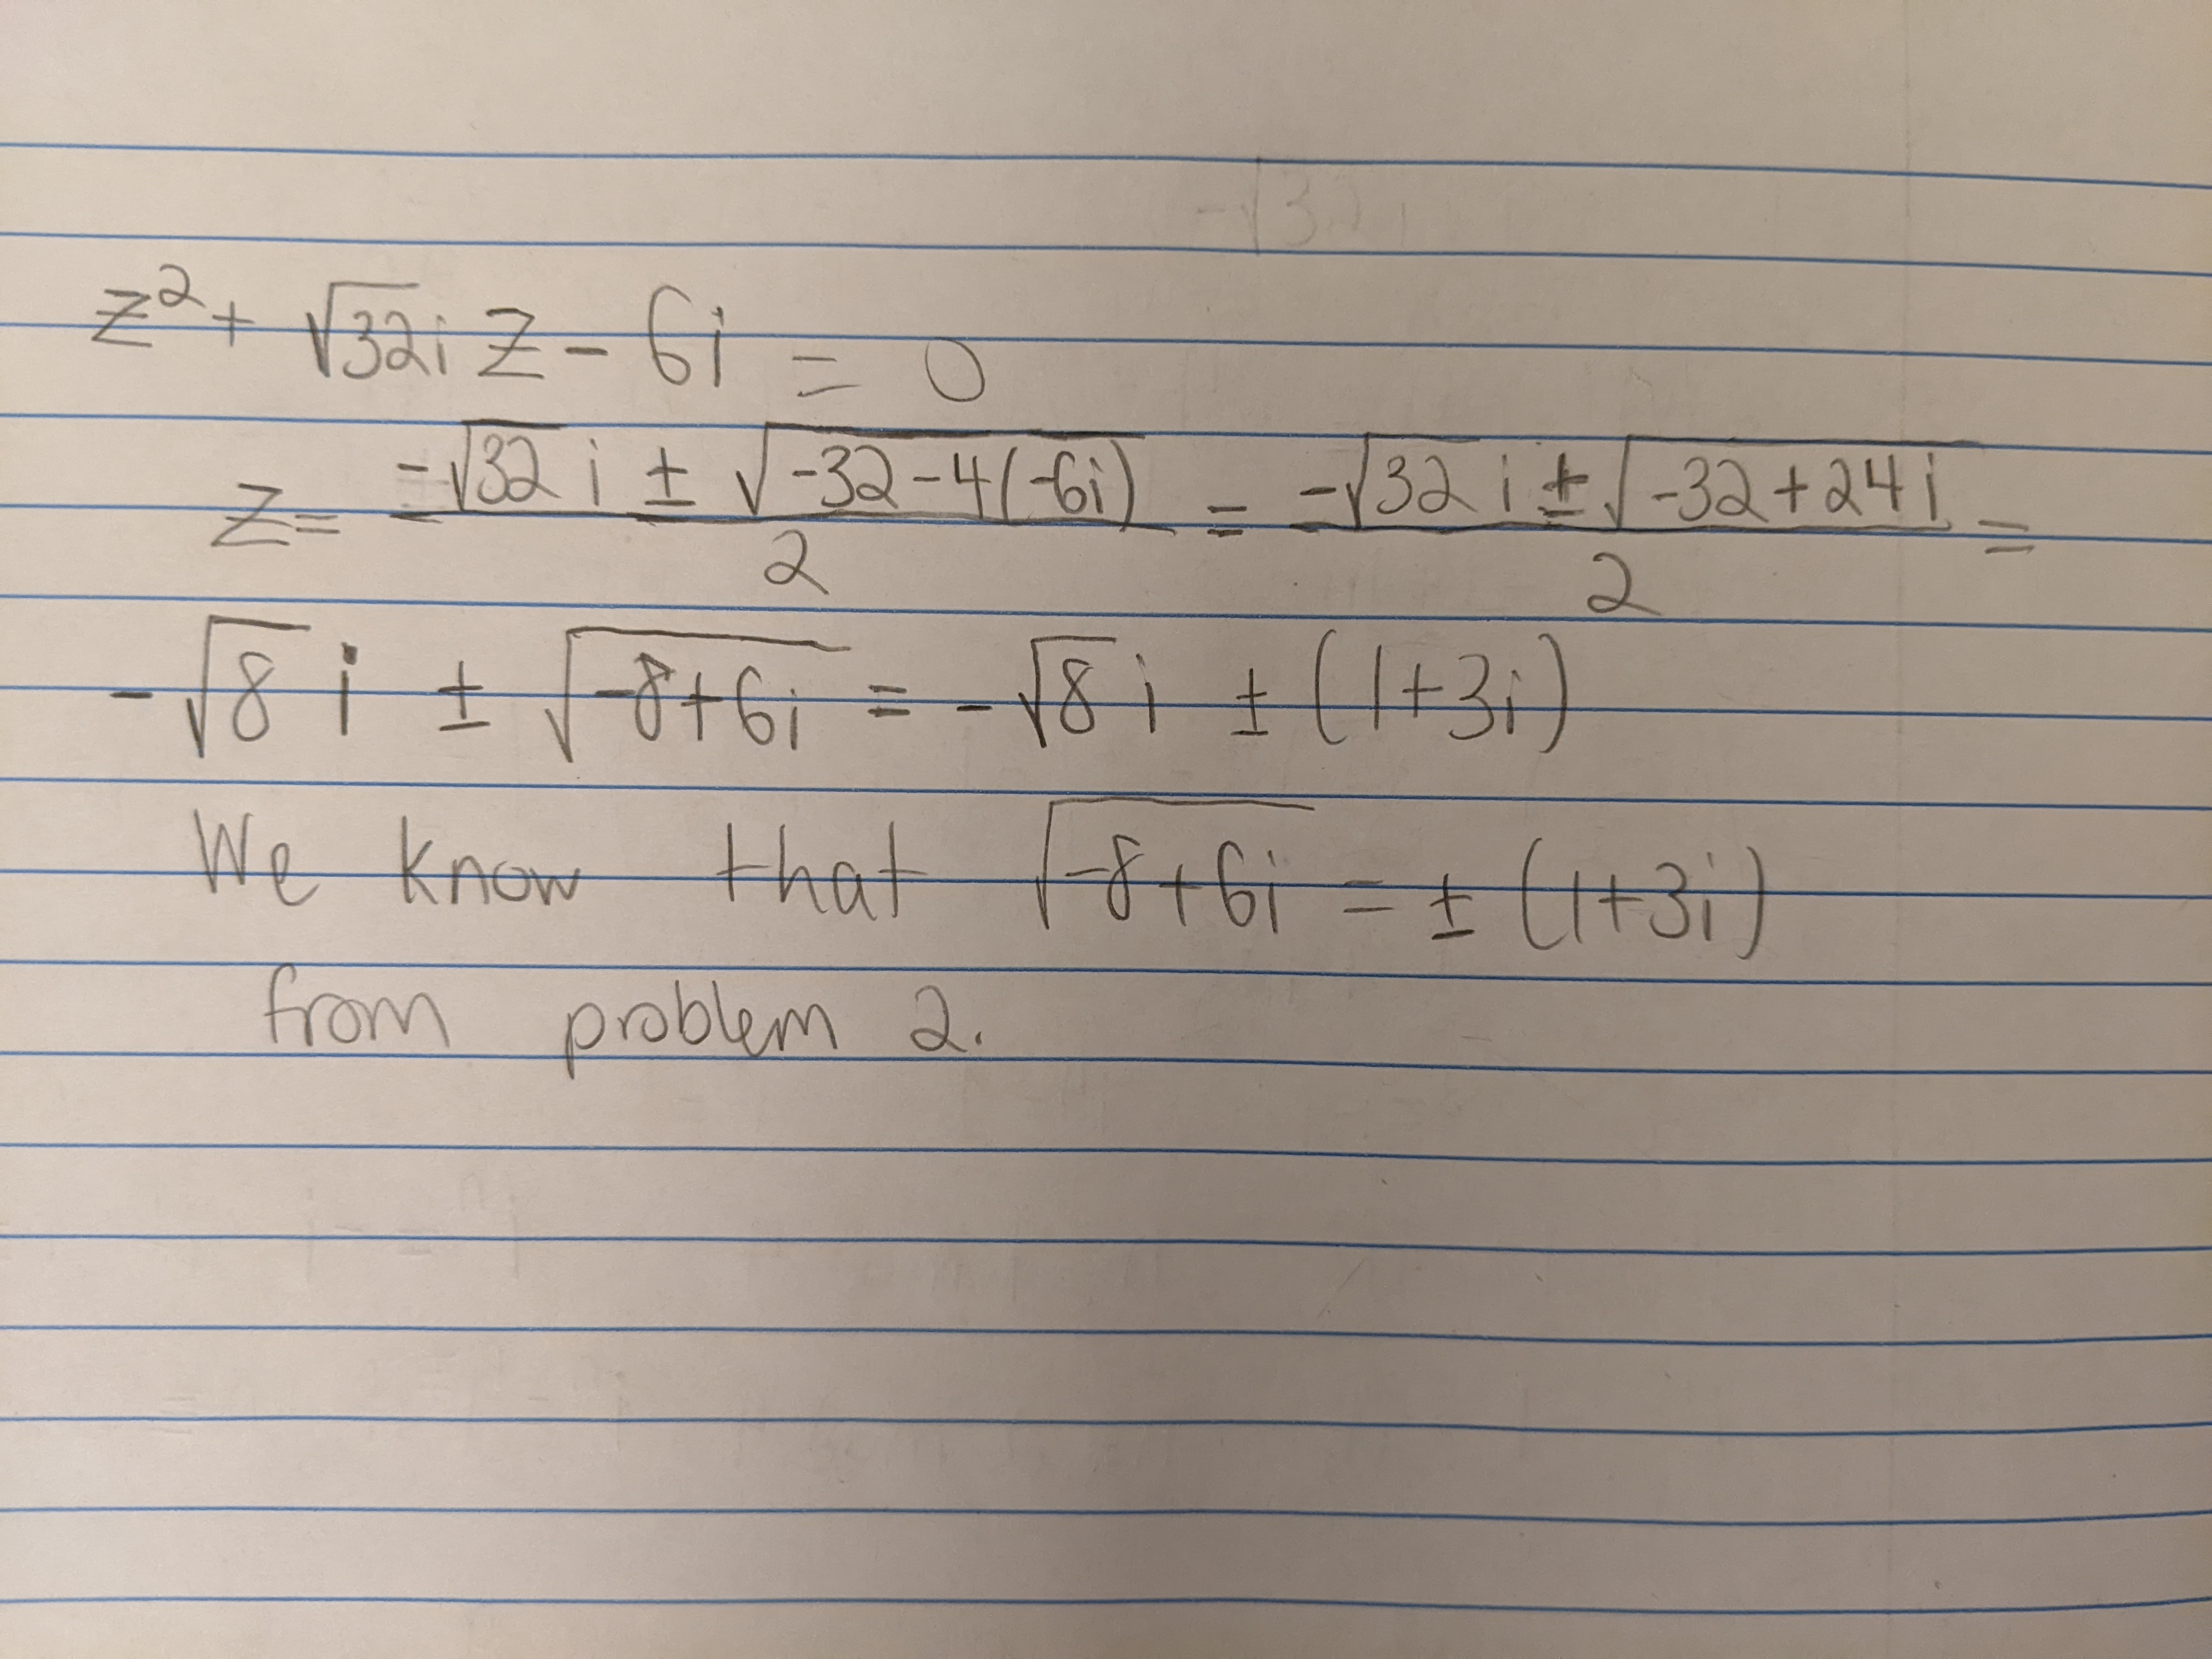
\includegraphics[width=\textwidth]{3}
\end{figure}
\newpage
\section*{Problem 8}
\subsection*{Part A}
To show that \[\vert z_1 + z_2\vert^2 = (z_1 + z_2)(\overline{z_1}+ \overline{z_2})\] we note that $\vert z_1 + z_2 \vert ^2 = (z_1+z_2)(\overline{z_1+z_2})$ by the definition of modulus and that $\overline{z_1+z_2} = \overline{z_1} + \overline{z_2}$ by the properties of conjugation. By appealing to the distributive property and the definition of modulus, we find that
\[
(z_1 + z_2)(\overline{z_1}+ \overline{z_2}) = \vert z_1 \vert^2 + \vert z_2 \vert ^2 + z_1\overline{z_2} + \overline{z_1}z_2
\] Next, we note that $\overline{z_1}z_2 = \overline{z_1\overline{z_2}}$ so that $z_1\overline{z_2} + \overline{z_1}z_2 = z_1\overline{z_2} +  \overline{z_1\overline{z_2}} = 2 \re(z_1\overline{z_2})$ by the properties of conjugation. This shows that
\[
\vert z_1 \vert^2 + \vert z_2 \vert ^2 + z_1\overline{z_2} + \overline{z_1}z_2 = \vert z_1 \vert^2 + \vert z_2 \vert ^2 + 2\re(z_1 \overline{z_2})
\] Next, we note that $\re(z_1\overline{z_2}) \leq \vert z_1\overline{z_2} \vert$ because the modulus of any number is always greater than or equal to the real or imaginary part of that number. Note that $\vert z_1\overline{z_2} \vert = \vert z_1 \vert \vert \overline{z_2} \vert = \vert z_1 \vert \vert z_2 \vert$ because the modulus of the product is equal to the product of the moduli (and $\vert z \vert = \vert \overline{z} \vert$ because the modulus of a number is equal to the modulus of its conjugate). Thus, we obtain 
\[
\vert z_1 \vert^2 + \vert z_2 \vert ^2 + 2\re(z_1 \overline{z_2}) \leq \vert z_1 \vert^2 + \vert z_2 \vert ^2 + \vert z_1 \vert \vert z_2 \vert
\] Finally, appealing to the distributive property, we find that
\[
 \vert z_1 \vert^2 + \vert z_2 \vert ^2 + \vert z_1 \vert \vert z_2 \vert = (\vert z_1 \vert + \vert z_2 \vert)^2
\] so that we ultimately obtain
\[
\vert z_1 + z_2 \vert ^2 \leq (\vert z_1 \vert + \vert z_2 \vert)^2
\] Taking square roots yields
\[
\vert z_1 + z_2 \vert \leq \vert z_1 \vert + \vert z_2 \vert
\] as desired.
\subsection*{Part B}
Note that this triangle inequality is an inequality because $\re(z_1\overline{z_2}) \leq \vert z_1 \overline{z_2} \vert$. In order for this to be an equality, we must have $\re(z_1\overline{z_2}) = \vert z_1 \overline{z_2} \vert$. This means that $z_1 \overline{z_2}$ must be real and positive. Let us write $z_1 = r_1\cis(\theta_1)$ and $z_2 = r_2\cis(\theta_2)$. Then we have
\[
z_1 \overline{z_2} = r_1r_2 \cis(\theta_1-\theta_2) = r_1r_2(\cos(\theta_1-\theta_2)+i\sin(\theta_1-\theta_2))
\] Since we know that $z_1 \overline{z_2}$ is real and positive, we must have $\theta_1 - \theta_2 = 0$ so that $\theta_1 = \theta_2$. This means that $z_1$ and $z_2$ must be scalar multiples of each other.
\subsection*{Part C}
By the triangle inequality, we have
\[
\vert z_1 \vert = \vert z_1 - z_2 + z_2 \vert \leq \vert z_1 - z_2 \vert + \vert z_2 \vert
\] which implies that
\[
\vert z_1 \vert - \vert z_2 \vert \leq \vert z_1 - z_2 \vert
\]
\newpage
\section*{Problem 10}
Note that $\vert z_1 + z_2 \vert^2  = (z_1+z_2)(\overline{z_1+z_2})$ by the definition of modulus. Appealing to the properties of conjugation, we find that
$(z_1+z_2)(\overline{z_1+z_2}) = (z_1+z_2)(\overline{z_1} + \overline{z_2}) =  \vert z_1 \vert^2 + \vert z_2 \vert ^2 + z_1\overline{z_2} + \overline{z_1}z_2$. Similarly, we note that $\vert z_1 - z_2\vert^2 = \vert z_1 \vert^2 + \vert z_2 \vert ^2  - z_1\overline{z_2} - \overline{z_1}z_2$. Adding this all together, we obtain
\[
\vert z_1 + z_2 \vert^2 + \vert z_1 - z_2\vert^2 =  \vert z_1 \vert^2 + \vert z_2 \vert ^2 + z_1\overline{z_2} + \overline{z_1}z_2 + \vert z_1 \vert^2 + \vert z_2 \vert ^2  - z_1\overline{z_2} - \overline{z_1}z_2 = 2 \vert z_1 \vert^2 + 2 \vert z_2 \vert^2 = 2(\vert z_1 \vert^2 + \vert z_2 \vert ^2)
\] As can be seen in the below image, this theorem states that the squares of all four sides of a parallelogram add to the squares of the two diagonals of the parallelogram.
\begin{figure}[H]
\centering
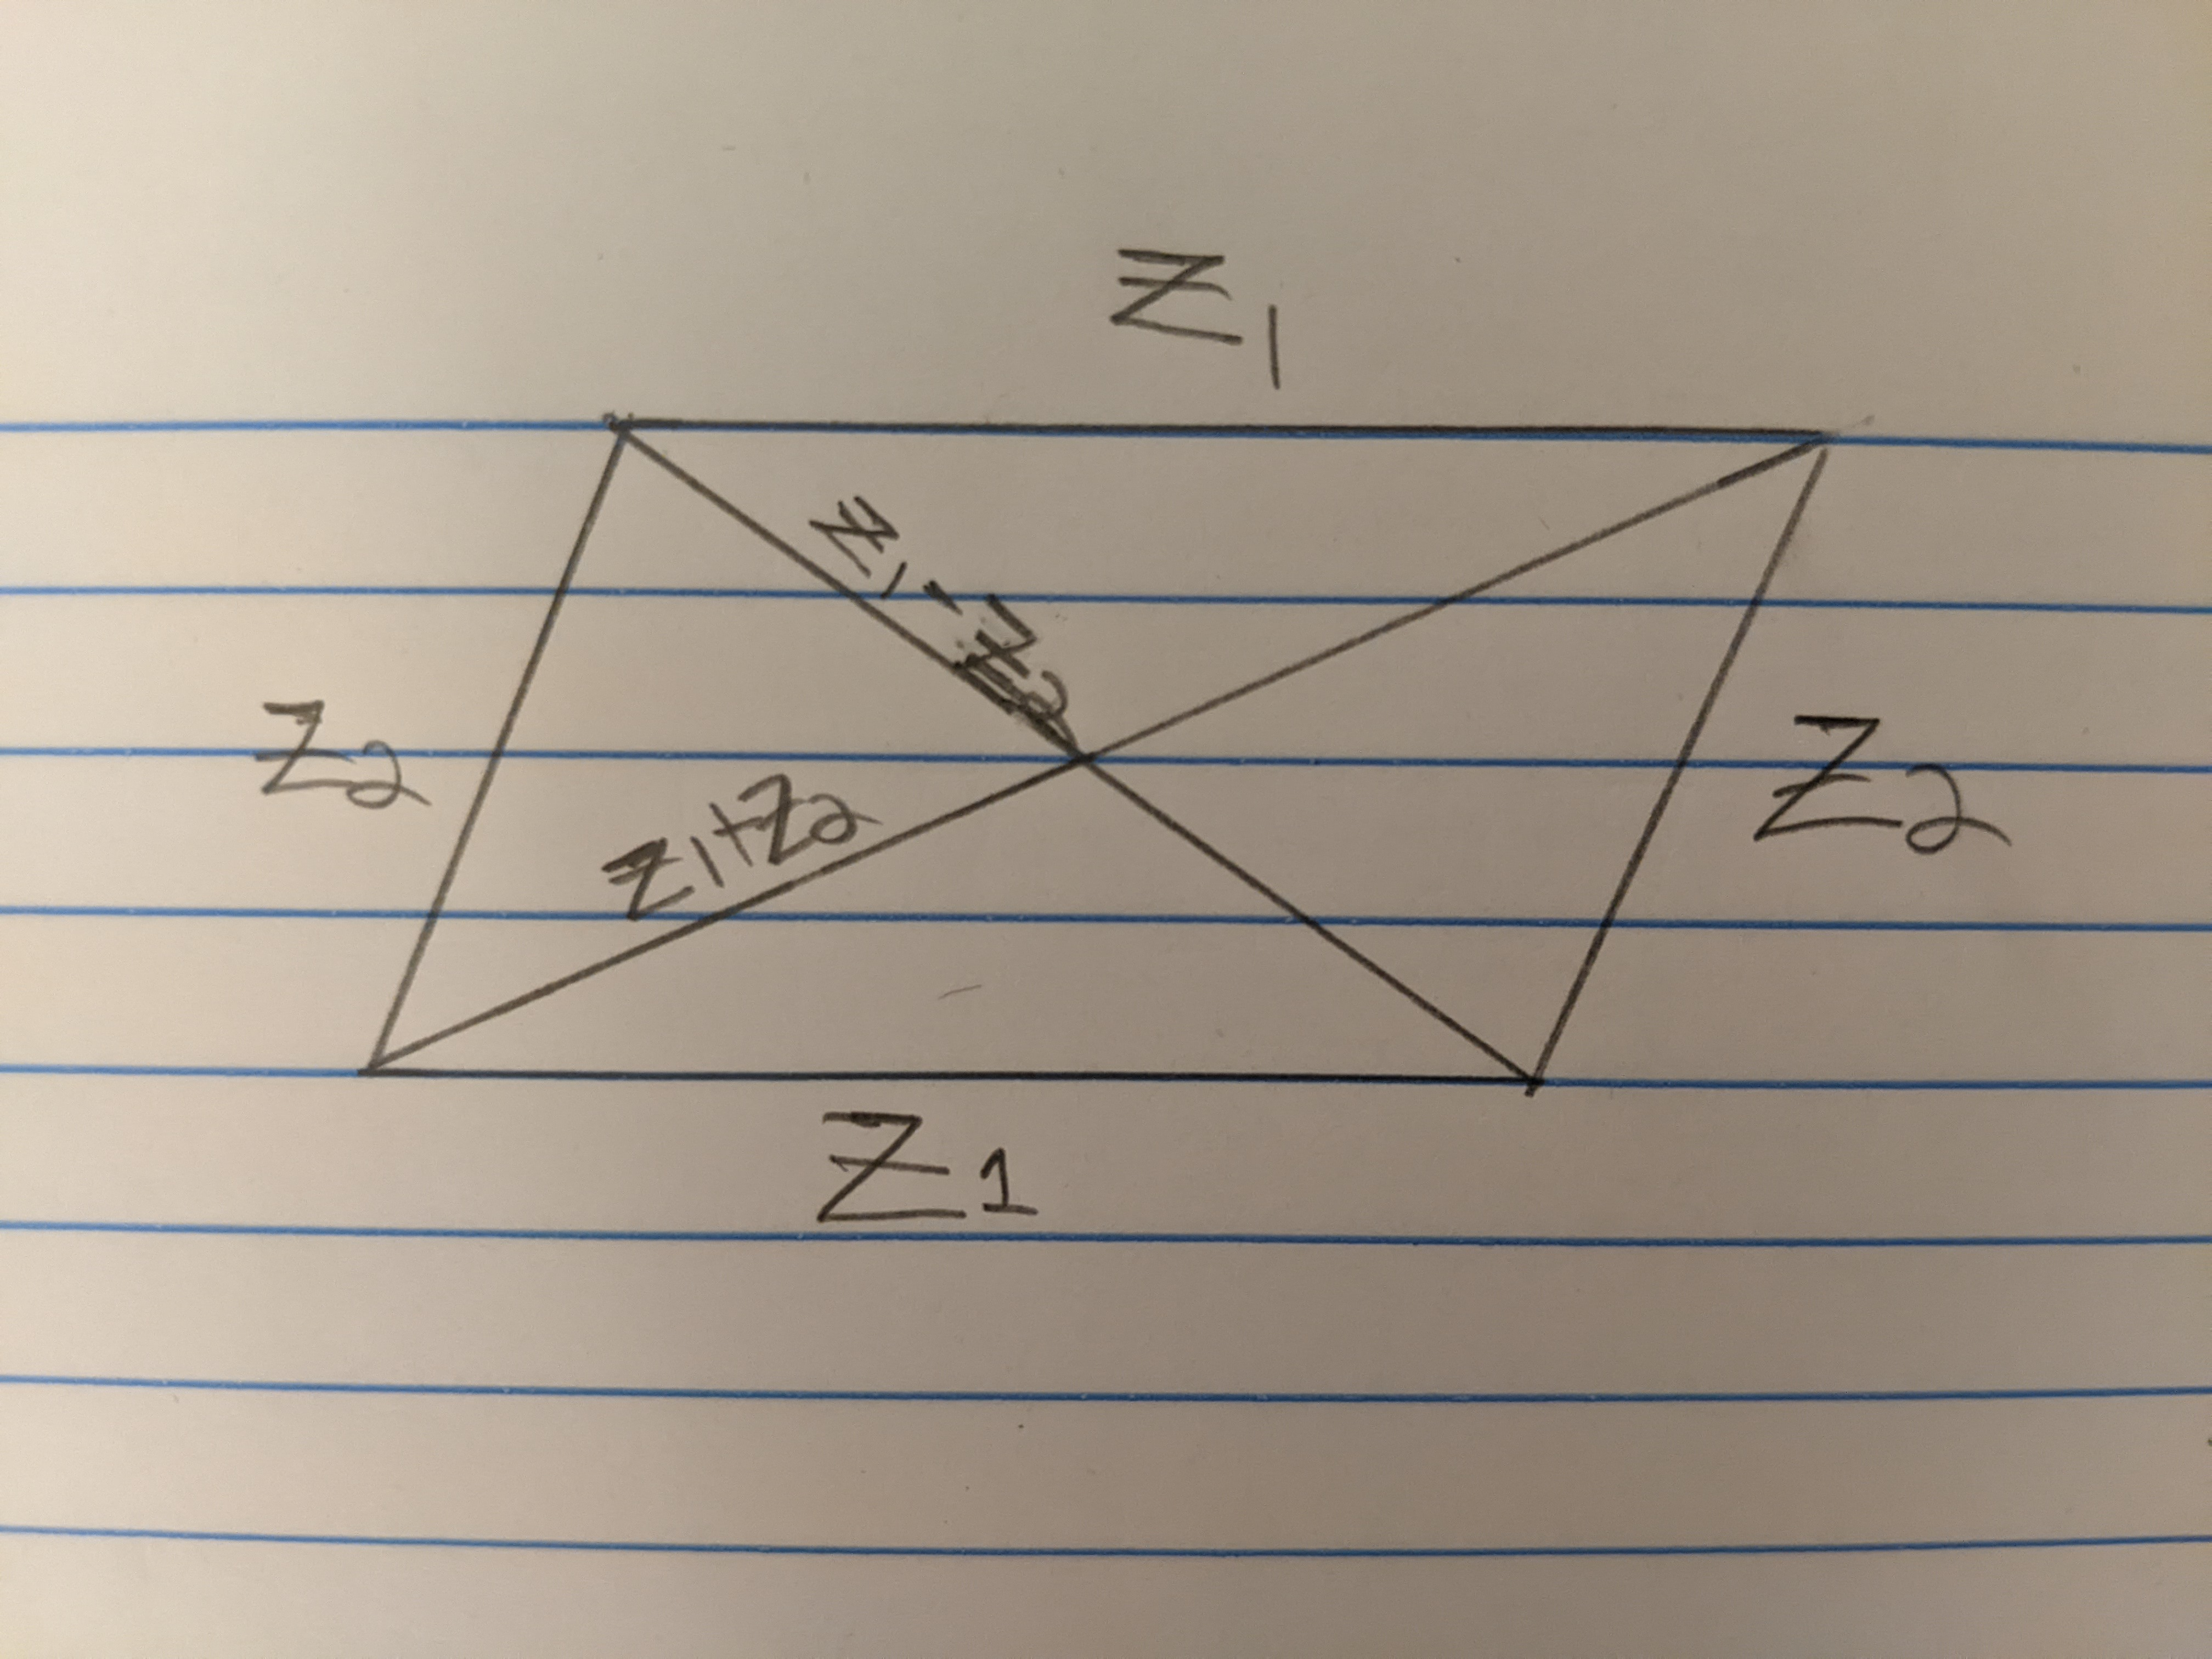
\includegraphics[width=\textwidth]{10}
\end{figure}
\newpage
\section*{Problem 12}
\subsection*{Part A}
We will solve $z^6 = 1$ in polar form. First, we may write this equation as $r^6 \cis 6\theta = 1 \cis 0$. This informs us that $r = 1$ and $6\theta=  0 \pmod{2\pi}$ Thus, we obtain the solutions $z_1 = 1$, $z_2 = \cis(\pi/3)$, $z_3 = \cis(2\pi/3)$, $z_4 = \cis(\pi)$, $z_5 = \cis(4\pi/3)$, and $z_6 = \cis(5\pi/3)$. These are the vertices of a regular hexagon inscribed in the unit circle with one of its vertices at $1$.
\subsection*{Part B}
We will solve $z^4 = -1$ in polar form. We may write this equation as $r^4 \cis 4\theta = 1 \cis (\pi)$. This informs us that $r = 1$ and $4\theta = \pi \pmod{2\pi}$. This means that $4\theta = \pi + 2\pi k$, where $k$ is an integer. Solving for $\theta$ yields $\theta = \pi/4 + \pi/2 \cdot k$. Thus, the solutions of this problem are $z_1 = \cis(\pi/4)$, $z_2 = \cis(3\pi/4)$, $z_3 = \cis(5\pi/4)$, and $z_4 = \cis(7\pi/4)$. These are the vertices of a square inscribed in the unit circle such that the sides of the square are parallel to the real and imaginary axes.
\subsection*{Part C}
We will solve $z^4 = -1 + \sqrt{3}i$ in polar form. Notice that $-1+\sqrt{3}i$ can be expressed in polar form as $2\cis (2\pi/3) $, so we have $r^4 \cis 4\theta = 2\cis (2\pi/3)$. We find that $r =  \sqrt[4]{2}$ and $4\theta = 2\pi/3 \pmod{2\pi}$. This informs us that $4\theta = 2\pi/3 + 2\pi k$ where $k$ is an integer. We obtain $\theta = \pi/6 + \pi/2 \cdot k$. The solutions are therefore $z_1 = \sqrt[4]{2} \cis(\pi/6)$, $z_2 = \sqrt[4]{2} \cis(2\pi/3)$, $z_3 = \sqrt[4]{2} \cis (7\pi/6)$, and $z_4=  \sqrt[4]{2}\cis(5\pi/3)$. These roots are the vertices of a square inscribed in a circle of radius $\sqrt[4]{2}$.
\end{document} 